%--------------------------------------------------------------------------
%
%                                                    SOLUTION
%
%--------------------------------------------------------------------------
\noindent {\large {\bf Saut du saumon}}\\[-3mm]
\begin{enumerate}
\item
On part de l'\'equation du mouvement
\[
\ddot{x}(t) =  a,
\] 
que l'on l'int\`egre une fois pour trouver la vitesse au cours du temps
\begin{equation}
\dot{x}(t) = at + cte.
\label{eq_premiereintegrale}
\end{equation}
Pour d\'eterminer \`a quoi correspond la constante d'int\'egration, on \'evalue l'expression (\ref{eq_premiereintegrale}) \`a l'instant $t=0$:
\[
\dot{x}(t=0) = 0 + cte. 
\]
La constante est donc \'egale \`a la vitesse \'evalu\'ee \`a l'instant $t=0$. On notera cette vitesse initiale $v_0$. 
On int\`egre une deuxi\`eme fois pour trouver la position au cours du temps
\begin{equation}
x(t) = \frac{1}{2}at^2 + v_0 t + cte'.
\label{eq_deuxiemeintegrale}
\end{equation}
On \'evalue ici encore cette expression en $t=0$ pour trouver \`a quoi correspond la constante d'int\'egration
\[
x(t=0) = 0 + 0 + cte'.
\]
La constante est \'egale \`a la position \'evalu\'ee en $t=0$. Il s'agit de la position initiale, not\'ee $x_0$.
Au final, la solution de l'\'equation du mouvement $\ddot{x}(t) =  a$ s'\'ecrit bien $x(t) = \frac{1}{2}at^2 + v_0 t + x_0$ o\`u $v_0$ et $x_0$ repr\'esentent respectivement la vitesse et la position initiales.

Pour v\'erifier que la solution $x(t)=\frac{1}{2}at^2+v_0t+x_0$ satisfait bien l'\'equation $\ddot{x}=a$ on calcule
\[
\ddot{x}(t) \equiv \frac{d^2x(t)}{dt^2} = \frac{d^2}{dt^2}\left(\frac{1}{2}at^2+v_0t+x_0\right)
\]
\[
= \frac{d}{dt}\left(\frac{1}{2}a2t+v_0\right) = \frac{d}{dt}\left(at+v_0\right) = a.  
\]
L'\'equation du mouvement rectiligne uniform\'ement acc\'el\'er\'e est donc bien v\'erifi\'ee.

\item \textbf{Compr\'ehension de l'\'enonc\'e:} La mani\`ere la plus efficace de comprendre le probl\`eme est de repr\'esenter la donn\'ee dans un \emph{grand} dessin comprenant toutes les indications de la donnée (voir ci-dessous). Le système que l'on considère est le saumon, et on l'observe depuis la bord du lac (référentiel). On choisit un axe $x$ vertical dirigé vers le haut, ayant son origine à la surface de l'eau.
 A l'instant $t=0$, le saumon sort du lac en $x_0=0$ avec une vitesse $v_0$ verticale, dirig\'ee vers le haut. Tout au long du saut, il subit une acc\'el\'eration $-g$ due \`a la pesanteur. Sa position au cours du temps est donn\'ee par l'\'equation (\eqref{eq_deuxiemeintegrale}) et sa vitesse au cours du temps par l'\'equation (\eqref{eq_premiereintegrale}) dans lesquelles on pose $a=-g$. 
\begin{center}
%\scalebox{1.2}{\input{figures//serie01_c_fig1.pdf_t}}\\
\hspace*{15mm}
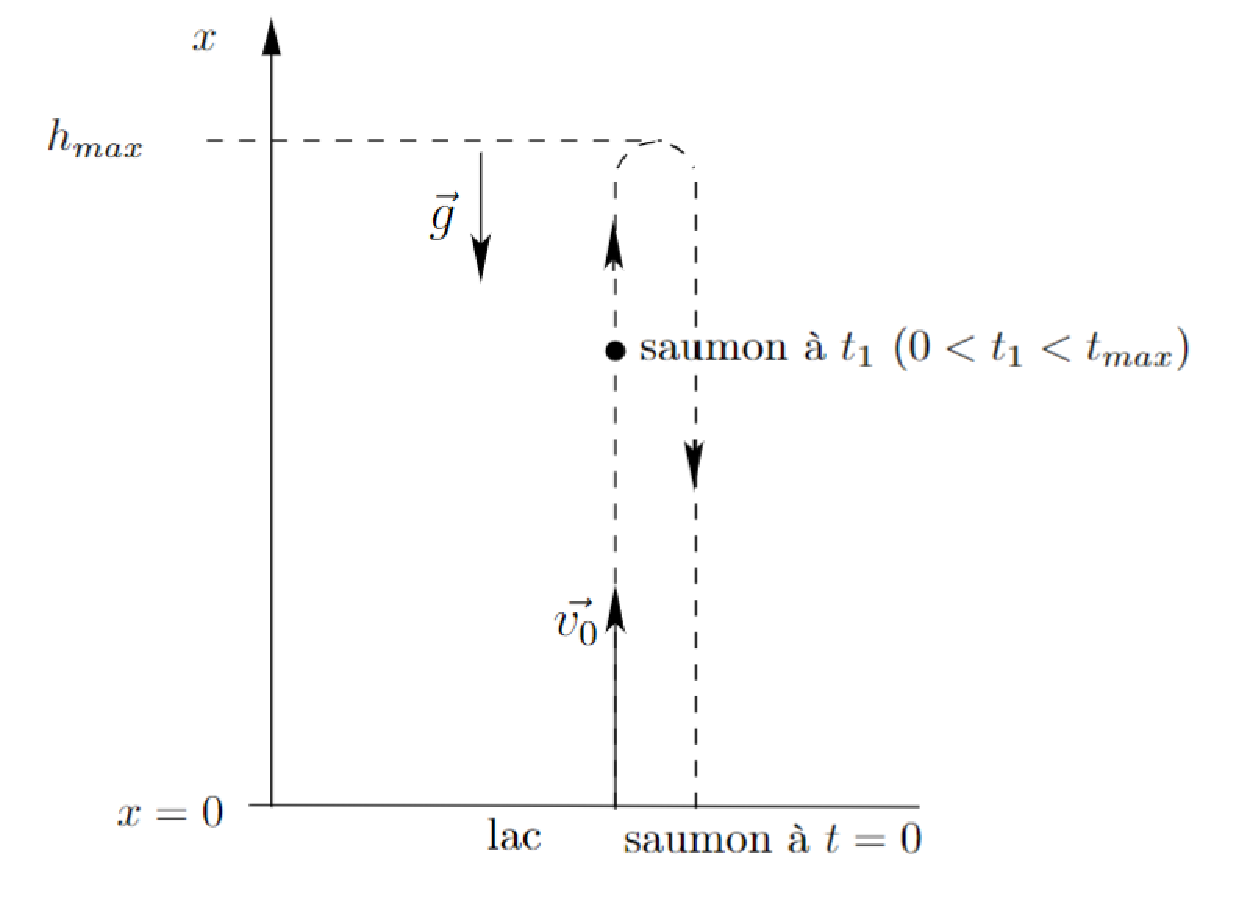
\includegraphics[width=10cm]{figures//serie01_c_fig1-2b.pdf}
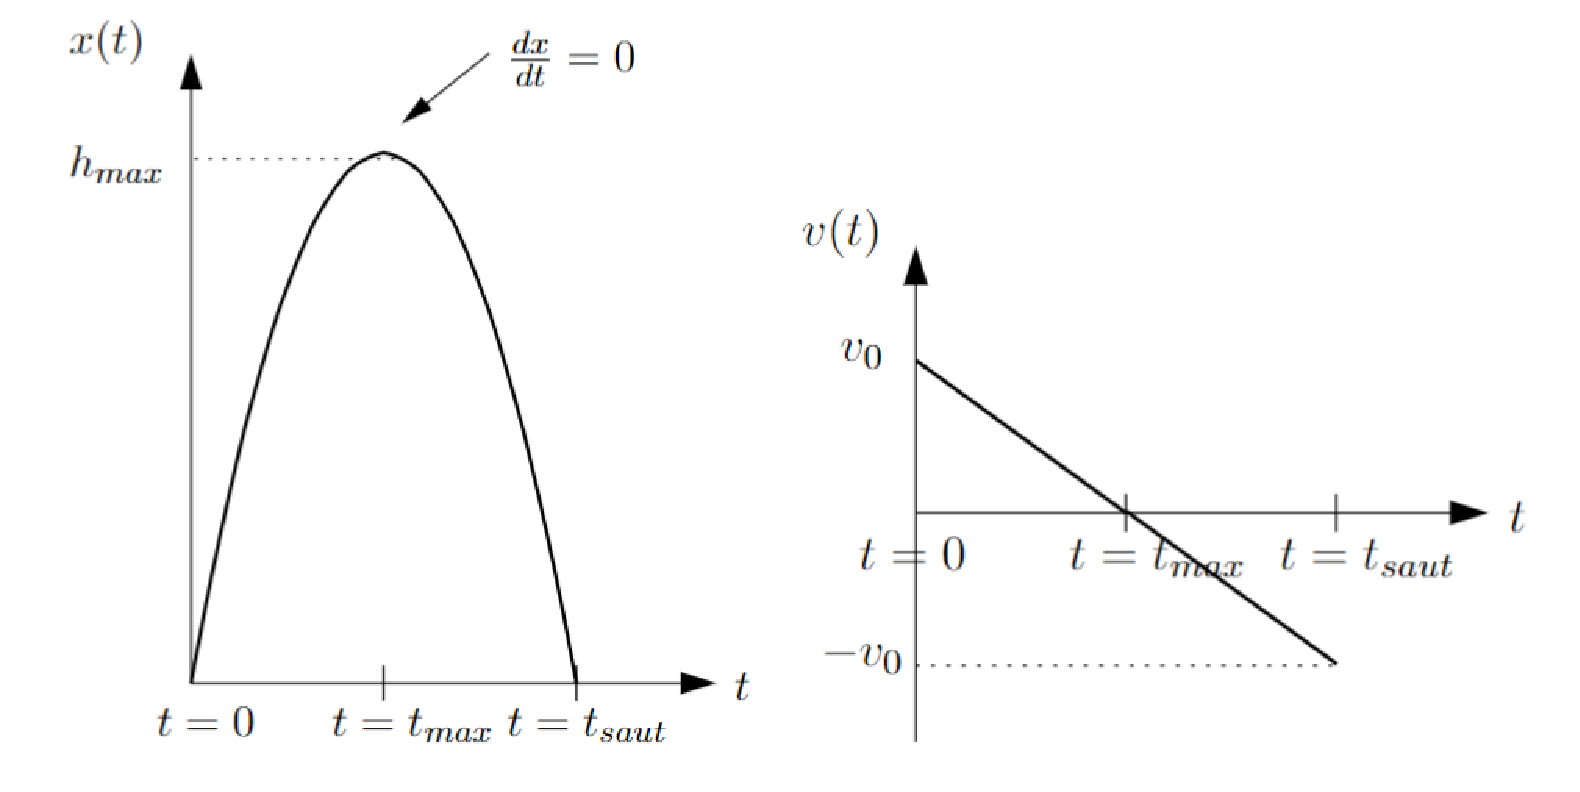
\includegraphics[width=14cm]{figures//serie01_c_fig1-2c.pdf}
\end{center}
\vspace{0.9cm}

Graphiquement, la position et la vitesse au cours du temps sont donn\'ees dans les deux figures ci-dessus. On peut remarquer que: 
\begin{itemize}
\item La position au cours du temps est donn\'ee par un polyn\^ome du deuxi\`eme degr\'e. Graphiquement, on a donc une parabole. 
\item Le sommet de la parabole correspond \`a l'altitude maximale atteinte par le saumon, \`a un instant que l'on nomme $t=t_{\rm max}$.
\item La vitesse diminue lin\'eairement. Graphiquement, elle est repr\'esent\'ee par une droite. La pente de cette droite est \'egale \`a l'acc\'el\'eration du saumon. 
\item A l'instant $t_{\rm max}$, la droite croise l'abscisse: la vitesse du saumon est nulle au sommet de la trajectoire. En tout point, la vitesse correspond \`a la d\'eriv\'ee de la position par rapport au temps. A l'instant $t_{\rm max}$, une vitesse nulle correspond donc au sommet de la parabole, de pente nulle. 
\item La parabole est sym\'etrique. Soit $t_{\rm saut}$ l'instant où le saumon retombe dans l'eau. On a $x(t_{\rm saut}) = 0$ et $t_{\rm max}= \frac{1}{2}t_{\rm saut}$.  
\end{itemize}
\item
\begin{itemize}
\item \textbf{D\'emarche(s) de r\'esolution:} On cherche \`a d\'eterminer la hauteur maximale atteinte par le saumon et le temps qu'il passera en l'air. Pour y arriver, la d\'emarche consiste \`a:
\begin{itemize}
% \item[-] Ecrire la deuxi\`eme \'equation de Newton $\Sigma \vec{F}_{ext} = m\vec{a}$ pour trouver l'acc\'el\'eration du saumon. 
\item[-] Int\'egrer une premi\`ere fois l'\'equation du mouvement $\ddot{x}(t)=a$ pour trouver la vitesse au cours du temps, puis une deuxi\`eme fois pour trouver la position au cours du temps.
\item[-] Utiliser les conditions aux limites pour r\'esoudre ces \'equations. \\
\end{itemize}
 \item \textbf{Choix d'une d\'emarche et r\'esolution:} 
% La seule force qui s'exerce sur le saumon est son poids $m\vec{g}$. La deuxi\`eme \'equation de Newton s'\'ecrit donc $m\vec{g} = m\vec{a}$. En projection sur l'axe vertical (voir dessin), on obtient $-mg = -ma \Rightarrow g = a$. \\
La premi\`ere partie de la d\'emarche a \'et\'e effectu\'ee dans la question a) de cet exercice. On utilise donc les \'equations (\eqref{eq_premiereintegrale}) et (\eqref{eq_deuxiemeintegrale}) pour lesquelles $a=-g$ et $x_0=0$:
\[
x(t) = -\frac{1}{2}gt^2 + v_0 t \quad \textrm{et} \quad v(t) = -gt + v_0. 
\]
Au sommet de la trajectoire (condition finale), le saumon atteint une hauteur $x(t_{\rm max}) = h_{\rm max}$ au temps $t_{\rm max}$. A cet instant, sa vitesse est nulle: $v(t_{\rm max})=0$. 
\[
-gt_{\rm max} + v_0=0 \Rightarrow t_{\rm max} = \frac{v_0}{g}.
\]
En injectant ce r\'esultat dans l'\'equation de la position au cours du temps, on obtient 
\[
h_{\rm max} = -\frac{1}{2}gt_{\rm max}^2 +v_0 t_{\rm max} = -\frac{1}{2}g\frac{v^2_0}{g^2} +v_0 \frac{v_0}{g} = \frac{1}{2}\frac{v_0^2}{g}.
\]
On calcule $t_{\rm saut}$ en utilisant la condition finale $x(t_{\rm saut}) = 0$:
\[
-\frac{1}{2}gt_{\rm saut}^2 + v_0t_{\rm saut}=0 \Rightarrow t_{\rm saut}=0 \mathrm{(solution\; \grave{a}\;\acute{e}viter)\;ou}\;t_{\rm saut} = \frac{2v_0}{g}.
\]
Ce r\'esultat confirme que $t_{\rm max} = \frac{1}{2}t_{\rm saut}$, comme on s'y attendait. \\

\emph{Application numérique:} \\
$v_0=3 \text{m/s}$ et $g=10 \text{m/s$^{2}$}$ donc $t_{\rm saut} = \frac{2v_0}{g} = \frac{2\times 3}{10}=0.6\,{\rm s}$ et $h_{\rm max} = \frac{1}{2}\frac{v_0^2}{g} = \frac{3^2}{2\times10}=0.45\,{\rm m}$. \\

\item \textbf{Discussion des solutions:} La solution trouv\'ee\ldots\\
\begin{itemize}
\item[-] \ldots a les bonnes unit\'es: pour $t_{\rm saut}$, on s'attend \`a un r\'esultat en secondes. $\frac{2v_0}{g} \rightarrow \frac{m/s}{m/s^2} = \frac{m}{s}\frac{s^2}{m} = s$. \\
Pour $h_{\rm max}$, on s'attend \`a un r\'esultat en m\`etres. $\frac{1}{2}\frac{v_0^2}{g} \rightarrow \frac{(m/s)^2}{m/s^2} = \frac{m^2}{s^2}\frac{s^2}{m} = m$. \\
\item[-] \ldots a le bon ordre de grandeur: $v_0 \simeq 10^0$ m/s et $g \simeq 10^1$ m/s$^2$. On a donc $t_{\rm saut} = \frac{2v_0}{g} \simeq \frac{10^0}{10^1} \simeq 10^{-1}$ s et $h_{\rm max} = \frac{1}{2}\frac{v_0^2}{g} \simeq \frac{10^0}{10^1} \simeq 10^{-1}$ m. Il para\^it effectivement raisonnable que le saumon saute \`a quelques dizaines de centim\`etres et que ce saut dure quelques  dixi\`emes de secondes. \\
\item[-] \ldots a les bons signes: $h_{\rm max}$ doit \^etre positif, car il se situe \`a une valeur positive sur l'axe vertical (voir dessin). On a bien $\frac{1}{2}\frac{v_0^2}{g} > 0$. De plus, $t_{\rm saut}$ doit \^etre positif, car le saumon retombe dans l'eau apr\`es avoir saut\'e. On a bien $\frac{2v_0}{g}$ > 0. \\
\item[-] \ldots est coh\'erente avec les cas limites. Si $v_0 \to \infty$ (le saumon saute avec une tr\`es grande vitesse) on a $h_{\rm max} \to \infty$ (il atteint une hauteur tr\`es importante) et $t_{\rm saut}\to \infty$ (ce saut dure un temps tr\`es long). On peut faire un raisonnement similaire avec $v_0 \to 0$. \\
\end{itemize}
\end{itemize}

\end{enumerate}




